%\documentclass[german]{exercise}
%\documentclass[german,answers]{exercise}
%\documentclass[additions]{bs-exercise}
\documentclass[german,additions,answers]{exercise}


%%%%%%%%%%%%%%%%%%%%%%%%%%%%%%%%%%%%%%%%%%%%%%%%%%%%%%%%%%%%%%%%%%%%%%%%
\bsauthor{Granitzer}
\bsyear{2013}
\bsreadingtitle{Medientechnik}


%%%%%%%%%%%%%%%%%%%%%%%%%%%%%%%%%%%%%%%%%%%%%%%%%%%%%%%%%%%%%%%%%%%%%%%%
\begin{document}

%%% 
\exerciseheader[\today]{�bungsblatt 3 - Digitalisierung - WS 13/14}


\begin{exercise}{Digitalisierung - Allgemeine Fragen}
\label{ex-de-mt-digitalisierung-fragen}
Beantworten sie folgende Fragen:
\begin{enumerate}
\item Erkl�ren Sie den Unterschied zwischen analogen und digitalen Signalen?
\item Wie erfolgt die Abtastung eines Signals?
\item Geben sie Beispiele f�r die Abtastung von Audio bzw. Bildsignalen hinsichtlich der Bezug- und Wertachsen.
\item Worin liegt der Vorteil/Nachteil digitaler Signale?
\item Was ist das Abtasttheorem und welcher Effekt entsteht bei der Verletzung von diesem?
\item Geben Sie Beispiele f�r Aliasing-Effekte aus dem Audio und Bildbereich an und skizzieren sie deren Entstehung.
\item Was sind Fourier-Reihen?
\item Was sind Sinusoide Funktionen und wie unterscheidet sich diese Repr�sentation von einer Repr�sentation in der komplexen Ebene? Welche Effekte hat dies auf die Interpretation der Fourier-Transformation?
\item Was ist das Fourier-Spektrum?
\item Wie unterscheidet sich die diskrete Fourier Transformation von der kontinuierlichen Fourier Transformation?
\item Was ist der Leck-Effekt?
\item Wozu ben�tigt man Fenster in der Diskreten-Fourier-Transformation?
\item Was ist ein Spectrogramm?
\answer{[Siehe Vorlesungsfolien}
\end{enumerate}
\end{exercise}

 %%% Wissensfragen


\begin{exercise}{Abtasttheorem - Aliasing Effekt - 3 Pkt}
\label{ex-de-mt-antialiasing}
Warum drehen sich in Kinofilmen die R�der von Kutschen oft scheinbar r�ckw�rts? Skizzieren sie den Effekt und erkl�ren sie den Zusammenhang zur Signalanalyse.

\answer{
\clearpage
Sch�nes Beispiel hier: \url{http://michaelbach.de/ot/mot_wagonWheel/index-de.html}\\

Speichenrad mit Aufnahme und unterschiedlichen Zeitzust�nden:\\
\bsfigure[scale=0.5]{figure/speichenrad-lsg}
}
\end{exercise}


%%% Local Variables: 
%%% mode: latex
%%% TeX-master: "exercise-de-digitalisierung"
%%% End: 



\begin{exercise}{Digitalisierung von analogen Signalen }
\label{ex-de-mt-gestaltprinzipien}
Gegeben sei folgendes periodisches Sinussignal:
$f(x)=sin(0.5\pi x)+sin(\pi x)+sin(2\pi x)$

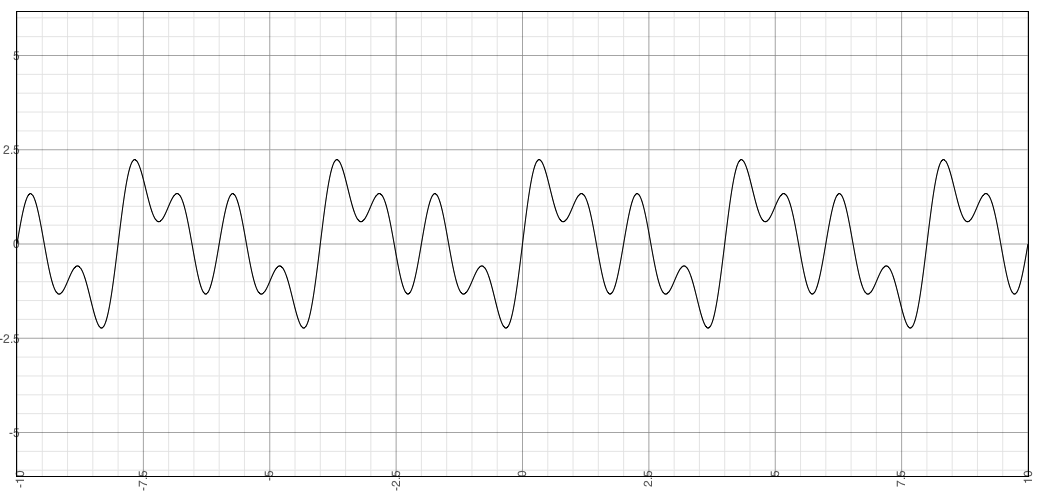
\includegraphics[width=0.8\textwidth]{figure/sin(05pix)+sin(2pix)+sin(pix)}

\begin{enumerate}
  \item Welche Frequenzen $f$ (bezogen auf den Einheitskreis) kommen im obigen Signal vor?
  \answer{
\clearpage
  $2\pi$ entspricht einer Kreisumdrehung in der Sekunde\\
  $2\pi f$ entspricht der Frequenz f (=Kreisumdrehungen pro Sekunde)\\
  $\rightarrow f_1=0.25,f_2=0.5,f_3=1 $
  }
  \item Geben sie 20 Digitalisierungswerte des abgetasteten Signals an, soda� dieses bei fortlaufender Abtastung rekonstruiert werden kann. Achten sie dabei darauf, nicht zu viele, unnotwendige Abtastwerte zu konstruieren.
\answer{
\clearpage
  Abtastfrequenz: $f_{abtast}>2*f_{max}=2*1 Hz$\\
  $sin(2\pi f_1 \mathbf{x})+sin(2\pi f_2 \mathbf{x})+sin(2\pi f_3 \mathbf{x})$, d.h. X-Achse ist
  in Sekunde\\
  Abtastung, mind. mit 2 Hz, d.h. 2 mal pro Sekunde. Der Einfachheit halber wird das Beispiel mit 4 mal pro Sekunde abgetastet (2.1 w�rde aber auch gen�gen).
  }
  \item Nehmen sie an, Ihnen stehen nur 3 Bit zur Speicherung eines Abtastwertes zu Verf�gung. Wie sieht das digitalisierte Signal aus? 
  \answer{
\clearpage
  3 Bit bedeutet 8 unterschiedliche Zust�nde, d.h. 4 in positiver und negativer Achse.
  Bei linearer Quantisierung stehen $\frac{4.9}{7}=0.7$ pro Quantisierungsstufe zu Verf�gung (1 Bit kodiert den Beginn)\\
  \bsfigure[scale=0.5]{figure/sin(05pix)+sin(2pix)+sin(pix)_lsg}
  \bsfigure[scale=0.5]{figure/sin(05pix)+sin(2pix)+sin(pix)_lsg2}
  }
  \item Gen�gen die 3-Bit zur vollst�ndigen Rekonstruktion des Signals?
  \answer{
\clearpage
  Nein. Bei der Quantsieriung erf�hrt die Digitalisierung immer einen Verlust.
  }   

  \item Wodurch unterscheidet sich die Funktion 
   $$f_{neu}(x)=sin(2\pi
    f_1 x+\pi/3)+sin(2\pi f_2 x+\pi/3)+sin(2\pi f_3
    x+7\pi/3)$$ vom Ursprungssignal $f(x)$.
   \answer{durch einen um $\pi/3$ fr\"uheren Start. Ansonsten ist das
     Signal identisch} 
\end{enumerate}

\end{exercise}


%%% Local Variables: 
%%% mode: latex
%%% TeX-master: "exercise-de-digitalisierung"
%%% End: 


\begin{exercise}{Fourier-Analyse - Sinus/Cosinus Koeffizienten }
\label{ex-de-mt-fourier}
Verwenden sie das Programm unter \url{http://www.fourier- series.com/fourierseries2/flash_programs/fourier_series_sin_cos/index.html} und erzeugen sie ein beliebiges Signal (Slider oben links).\\
Erkl�ren sie danach die Berechnung von
\begin{itemize}
  \item zwei Kosinuskoeffizienten
  \item zwei Sinuskoeffizienten
  \item der beiden Gleichanteil-Koeffizienten. 
\end{itemize}
unter Verwendung des Buttons "`Manually Calculate Basis Function Coefficients"' (rechts-unten). Ermitteln sie danach �ber die Funktion "`Automatically Calculate Basis Function Coefficients"' (rechts-unten) alle Koeffizienten und diskutieren sie die Effekte, wenn gewisse Koeffizienten nicht ber�cksichtigt werden. 
\end{exercise} 

\begin{exercise}{Fourier-Analyse }
\label{ex-de-mt-fourier-2}
\begin{itemize}
  \item Erkl�ren Sie kurz und ohne Formeln die Grundlagen und Funktionsweise von Fourierreihen (Fourierkoeffizienten und deren Bedeutung)
  \item Fourierreihen lassen sich eigentlich nur bei periodischen Signalen nutzen. Wie kann man diese Einschr�nkung umgehen und auch nichtperiodische Signale damit beschreiben?
  \item Skizzieren sie f�r eine reine Sinuskurve mit einer Frequenz von 1000Hz das Originalsignal sowie den Frequenzraum.
  \item Skizzieren sie den Frequenzraum f�r folgendes Signal: $f(x)=sin(8\pi x)+sin(2\pi x)+sin(200\pi x)$
  \item Ordnen sie die unten angef�hrten Signalverl�ufe (a-c) den entsprechenden Frequenzspektren (1-3) zu.\\[2ex]
  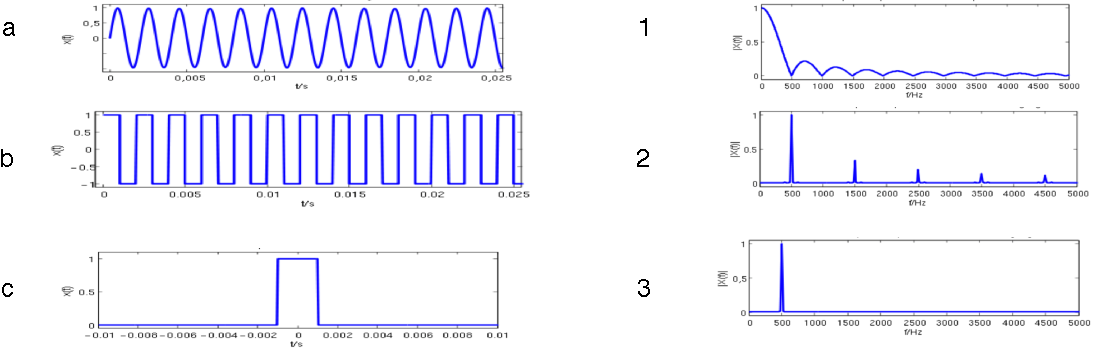
\includegraphics[width=0.8\textwidth]{figure/spektren}
\end{itemize} 
\end{exercise} 

\begin{exercise}{Fourier-Analyse - Sinusoide Repr�sentation }
\label{ex-de-mt-fourier-3}
Verwenden sie das Programm unter \url{http://www.fourier-series.com/fourierseries2/flash_ programs/four_freqs/index.html} zur Erzeugung Sinusoider Signale. 

Beantworten sie folgende Fragen
\begin{itemize}
  \item Erk�ren sie damit die Effekte von geraden und ungeraden Funktionen (Cosinus bzw. Sinus).
  \item Zeigen sie unter Ber�cksichtigung nur einer Sinus- und eines Cosinusfunktion die damit entstehende Phasenverschiebung Sinusoider-Funktionen.
  \item Stellen sie ein zusammengesetztes Signal unter Verwendung der Funktion "`PlayBoth"' nach. 
\end{itemize}
\end{exercise} 

\begin{exercise}{Fourier-Analyse - Fourier-Transformation }
\label{ex-de-mt-fourier-4}

Verwenden sie das Programm unter \url{http://www.fourier-series.com/f-transform/flash-programs/FourierTrans.html}.\\
Beantworten Sie unter zu Hilfenahme des Programms folgende Fragen:
\begin{itemize}
  \item Erkl�ren sie die Fourier-Transformation sowie den Unterschied zwischen Sinusoider und komplexer Repr�sentation.
  \item Warum ist der Imagin�eranteil bei einem um den Ursprung gespiegelten Rechteck-Signal immer 0?
  \item Vergleichen Sie die Spektren eines Rechtecks und einer Sinc Funktion. Was f�llt ihnen auf?
  \item Warum sind die Spektren verschiedener Signale kontinuierlich?
\end{itemize}
\end{exercise}

\begin{exercise}{Fourier-Analyse - Diskrete-Fourier-Transformation }
\label{ex-de-mt-fourier-4}

Verwenden sie das Programm unter \url{http://www.fourier-series.com/fourierseries2/flash_programs/DFT_windows/index.html}.\\
Beantworten Sie unter zu Hilfenahme des Programms folgende Fragen:
\begin{itemize}
  \item Worin liegt der Unterschied zwischen Real $Re(X(m))$ und
    Imagin\"arteil $Im(X(m))$
    der DFT und der Darstellung von  $\sqrt{Re(X(m))^2+Im(X(m))^2}$
  \item Erkl\"aren sie den Effekt, wenn die Anzahl der abgetasteten
    Werte nicht einer Periode des Signals entspricht. Was passiert?
  \item Was sind Fensterfunktionen und wie wirken sich diese aus?
  \item Was bedeuten Angaben in $dB$?
\end{itemize}
\end{exercise}

\begin{exercise}{Filter -Theorie }
\label{ex-de-mt-filter-1}

\begin{itemize}
\item Wodurch unterscheiden sich Digital Filter von Analog Filter und
  welche Arten von Digital Filter kennen Sie?
\item Was ist die Transferfunktion?
\item Erkl\"aren Sie den Prozess der diskreten Faltung und in welchem
  Zusammenhang dieser mit LTI Filter steht?
\end{itemize}
\end{exercise}

\begin{exercise}{Filter -Praxisbeispiel }
\label{ex-de-mt-filter-1}
Gegeben seien zwei diskrete Signale $x_1(t)$ und  $x_2(t)$ mit folgenden
Werten in den Sekunden $1-19$:\\
\begin{center}
  \begin{tabular}{ccc}
    Zeit[s]& $x_1(t)$    & $x_2(t)$   \\
    \hline
    1    & 0,95  & 0,95  \\
    2    & 0,59  & -0,59 \\
    3    & -0,59 & -0,59 \\
    4    & -0,95 & 0,95  \\
    5    & 0,00  & 0,00  \\
    6    & 0,95  & -0,95 \\
    7    & 0,59  & 0,59  \\
    8    & -0,59 & 0,59  \\
    9    & -0,95 & -0,95 \\
    10   & 0,00  & 0,00  \\
    11   & 0,95  & 0,95  \\
    12   & 0,59  & -0,58 \\
    13   & -0,59 & -0,59 \\
    14   & -0,95 & 0,95  \\
    15   & 0,00  & 0,01  \\
    16   & 0,95  & -0,95 \\
    17   & 0,59  & 0,58  \\
    18   & -0,58 & 0,59  \\
    19   & -0,95 & -0,95 \\
  \end{tabular}
\end{center}
\begin{itemize}
\item Laden sie die Werte in ein Spreadsheet Programm wie
  z.B. Excel. Analysieren Sie die beiden Signale und errechnen Sie das
  Summensignal $s(t)=x_1(t)+x_2(t)$. Was kann man \"uber die Eigenschaften der
  Signale sagen?
\item  Realisieren Sie einen Mittelwertefilter 1. Ordnung. Welches
  Signal k\"onnen Sie aus $s(t)$ mit diesem Filter rekonstruieren und
  wie gut ist die Rekonstruktion?
  Vergleichen Sie verschiedene Filterkoeffizienten miteinander.
\item  Realisieren Sie einen Mittelwertefilter 2. Ordnung. Welches
  Signal k\"onnen Sie aus $s(t)$ mit diesem Filter rekonstruieren?
  Vergleichen Sie verschiedene Filterkoeffizienten miteinander und
  \"uberlegen Sie, wie man eine Phasenverz\"ogerung verhindern oder
  erzwingen kann. \"Andert sich die Ordnung des Filters?
\item  Realisieren Sie einen Hochpass 1. Ordnung, sodass $x_2(t)$ aus $s(t)$
  rekonstruiert werden kann.  Vergleichen Sie verschiedene Filterkoeffizienten miteinander und
 erkl\"aren Sie die Funktionsweise des Hochpass.
\item  Realisieren Sie einen IIR Filter 1. Ordnung.  Vergleichen Sie
  verschiedene Filterkoeffizienten miteinander und zeigen Sie die
  Stabilit\"atsprobleme von IIR Filtern.
\end{itemize}
\answer{see filter-excel.xls}
\end{exercise}
\end{document}
 

%%%%%%%%%%%%%%%%%%%%%%%%%%%%%%%%%%%%%%%%%%%%%%%%%%%%%%%%%%%%%%%%%%%%%%%%
 